\begin{document}

\chapter{Preparation}

The Preparation chapter presents the fundamental theory which serves as bases on which the algorithms in this project are developed. It explores the requirement analysis and software engineering strategies such that the project successfully achieves and (possibly) surpasses the success criteria. All the work described in this chapter is prior to any actual implementation.


\section{Introduction to Neural Networks}

An Artificial Neural Network (ANN) is a computational model that is inspired by the way biological neural networks in the human brain process information. Artificial Neural Networks have generated a lot of excitement in Machine Learning research and industry, thanks to many breakthrough results in speech recognition, computer vision and text processing.

\subsection{Artificial Neuron}

The basic unit of computation in a NN is the Artificial Neuron. A neuron receives input either directly from the dataset or from another neuron and combines it with a set of coefficients, known as weights, thereby assigning significance to inputs with regard to the task the algorithm is trying to learn. These input-weight products are summed and then passed through an activation function $\sigma : \mathbb{R} \rightarrow \mathbb{R}$ as can be observed in Figure \ref{Artificial Neuron}. The additional bias that is generated by each neuron allows shifting the activation function to the left or to the right. \\

\begin{figure}[H]
  \centering
  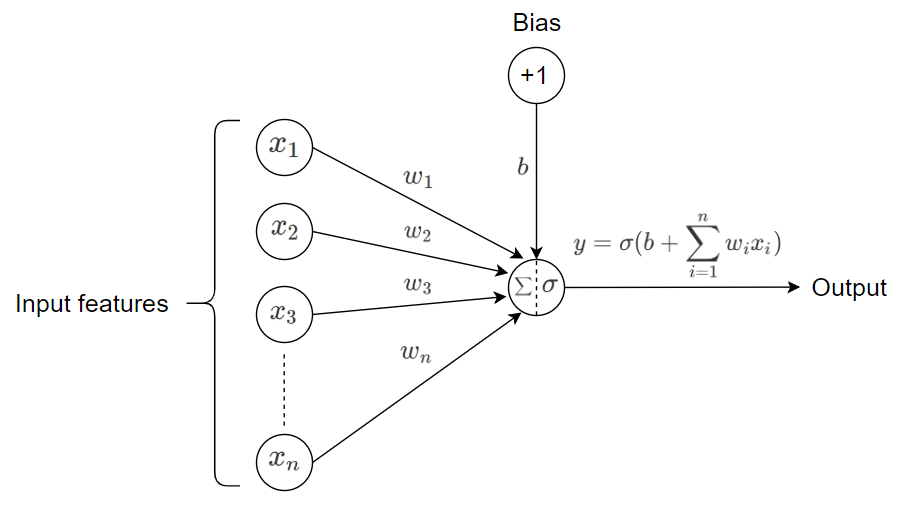
\includegraphics[scale = 0.5]{Images/artificial_neuron.png}
  \caption{Artificial Neuron Structure.}
  \label{Artificial Neuron}
\end{figure}

The purpose of an activation function is to introduce non-linearity into a NN, in the sense that the output will not be always represented as a linear combination of the inputs. Hence, it increased the expresivity and the diversity of functions that can be learnt by a NN. Some popular activation functions are listed below:\\

\begin{itemize}
  \item the sigmoid/logistic function: \\
        \begin{equation}
          \sigma(x) = \frac{1}{1 + e^{-x}}
        \end{equation}

  \item the hyperbolic tanget function: \\
        \begin{equation}
          \sigma(x) = tanh(x) = \frac{e^{x} - e^{-x}}{e^{x} + e^{-x}}
        \end{equation}

  \item the Rectified Linear Unit (ReLU) function: \\
        \begin{equation}
          \sigma(x) = max(0,x)
        \end{equation}
\end{itemize}


\subsection{Multilayer Perceptron}

A Multilayer Perceptron (MLP) is a finite, directed, acyclic graph in which the nodes represent artificial neurons and they are arranged in at least three layers. Nodes that are no target of any connection are called input neurons and represent input features. Nodes that are no source of any connection are called output neurons and represent predictions for the possible classes. Nodes that are neither input nor output neurons are called hidden neurons. The organisation of nodes in layers implies that nodes belonging to layer $i$ in the MLP serve as input features for nodes in layer $i+1$. \\

The most distinctive feature of MLPs is that they are fully connected NNs: each node in layer $i$ is connected to each node in layer $i+1$.

\begin{figure}[H]
  \centering
  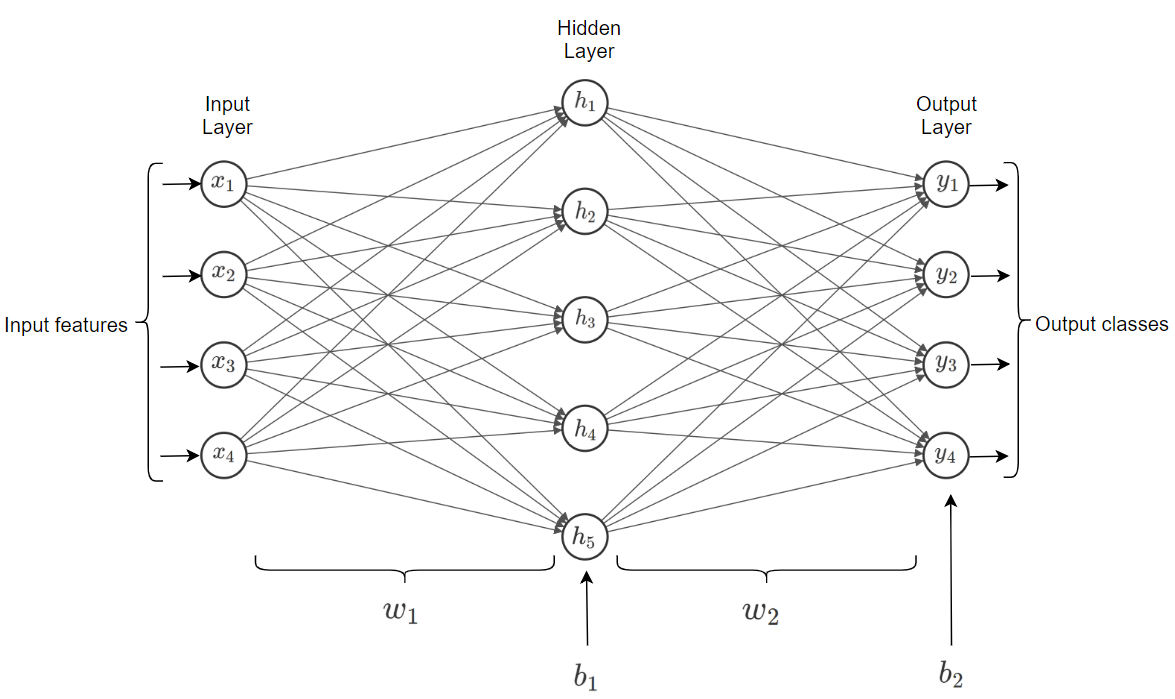
\includegraphics[scale = 0.5]{Images/mlp.png}
  \caption{Multilayer Perceptron Structure.}
  \label{Multilayer Perceptron}
\end{figure}

\subsection{Convolutional Neural Networks}

For some types of data, especially for images, MLPs are not the most appropriate approach. Indeed, they are defined on vectors as input data, which means, we shall transform images into vectors in order to apply MLPs, loosing the way spatial information is contained. \\\

In contrast to the baseline model of MLP, a Convolutional Neural Network (CNN) uses a specialised architecture (applied directly on matrices), well-adapted for image classification. A CNN is able to successfully capture the spatial dependencies in an image through the application of relevant filters. The architecture performs an adequate fitting to an image dataset due to the reduction in the number of parameters involved and re-usability of weights. A typical CNN is comprised of convolutional, pooling and dense layers. \\

\subsubsection*{Convolutional Layers}

Convolution is a specialised type of linear operation used for feature extraction, where a small array of numbers, called a kernel, is applied across the input, which is an array of numbers, called a tensor. An element-wise product between each element of the kernel and the input tensor is calculated at each location of the tensor and summed to obtain the output value in the corresponding position of the output tensor, called a feature map. This is illustrated in Figure \ref{Convolution}. This procedure is repeated applying multiple kernels to form an arbitrary number of feature maps, which represent different characteristics of the input tensors; different kernels can, thus, be considered as different feature extractors. The first convolution layer extracts low-level features like edges, lines, and corners. Higher-level layers extract higher-level features. \\

\begin{figure}[H]
  \centering
  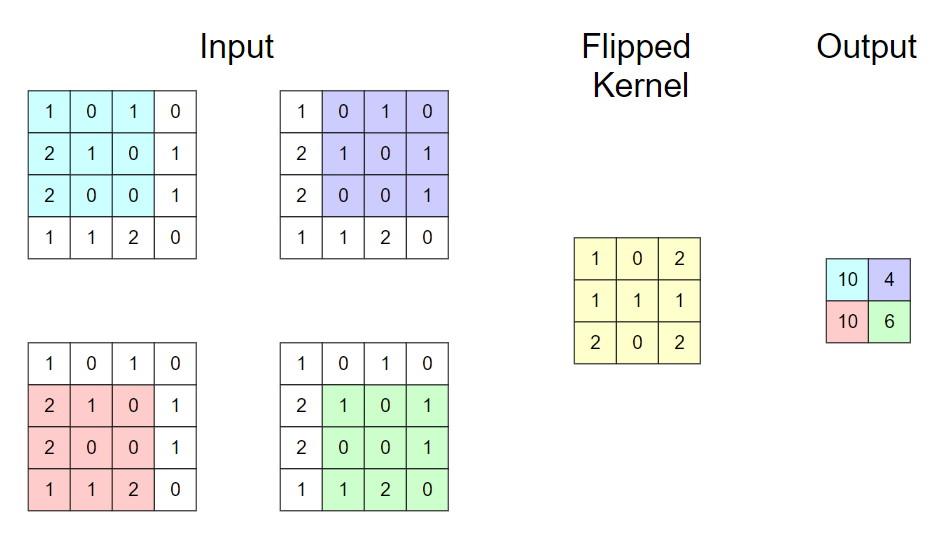
\includegraphics[scale = 0.6]{Images/convolution.png}
  \caption{Example of a Convolution operation where coloured areas of the input matrix are successively dot producted with the flipped kernel.}
  \label{Convolution}
\end{figure}

Formally, given the image size N*M and the kernel size L1*L2, the 2D discrete convolution is described by the following equation: \\

\begin{equation}
  \text{Convolution}_{ij} = \sum_{l_1=0}^{L1-1} \sum_{l_2=0}^{L2-1} K[l_1][l_2]*I[i+l_1][j+l_2]
\end{equation}
$$\text{where} \ 0 \leq i < N \ \text{and} \ 0 \leq j < M$$ \\

The convolution operation described above does not allow the center of each kernel to overlap the outermost element of the input tensor, and reduces the height and width of the output feature map compared to the input tensor. Padding, typically zero padding, is a technique to address this issue, where rows and columns of zeros are added on each side of the input tensor, so as to fit the center of a kernel on the outermost element and keep the same in-plane dimension through the convolution operation. \\

The key feature of a convolution operation is weight sharing: kernels are shared across all the image positions. Weight sharing creates the following characteristics of convolution operations: (1) letting the local feature patterns extracted by kernels translation b invariant as kernels travel across all the image positions and detect learned local patterns, (2) learning spatial hierarchies of feature patterns by subsampling in conjunction with a pooling operation, resulting in capturing an increasingly larger field of view, and (3) increasing model efficiency by reducing the number of parameters to learn in comparison with fully connected neural networks. \\


\subsubsection*{Pooling Layers}

Pooling is a procedure that reduces the input over a certain area to a single value (subsampling). An illustration of pooling can be found in Figure \ref{Pooling}. In convolutional neural networks, this concentration of information provides similar information to outgoing connections with reduced memory consumption. Pooling provides basic invariance to rotations and translations and improves the object detection capability of convolutional networks. For example, the face on an image patch that is not in the center of the image but slightly translated, can still be detected by the convolutional filters because the information is funneled into the right place by the pooling operation. The larger the size of the pooling area, the more information is condensed, which leads to slim networks that fit more easily into memory. However, if the pooling area is too large, too much information is thrown away and predictive performance decreases. \\

\begin{figure}[H]
  \centering
  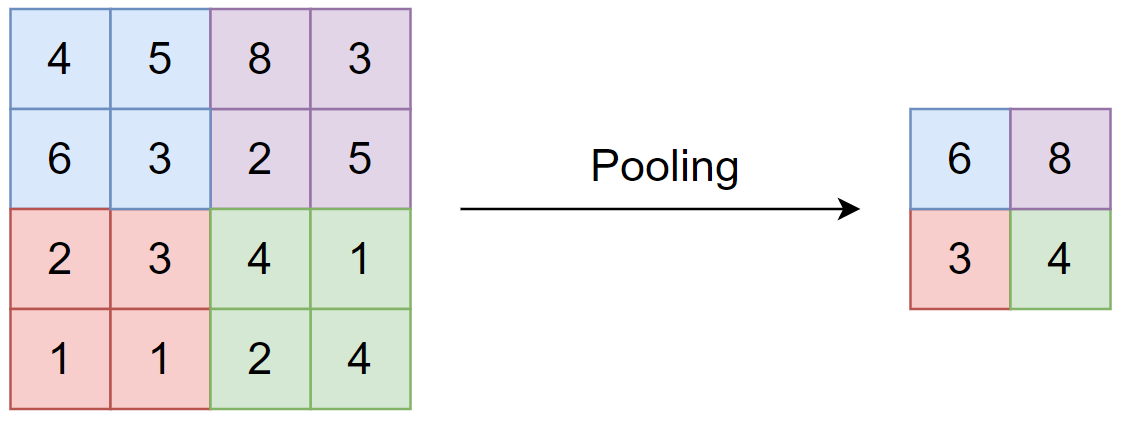
\includegraphics[scale=0.3]{Images/pooling.png}
  \caption{Example of Max Pooling operation with 2 by 2 kernel size and stride 2.}
  \label{Pooling}
\end{figure}

\subsubsection*{Fully Connected Layers}

After several convolution and pooling layers, the CNN usually ends with multiple fully connected layers. The output from the convolutional and pooling layers represent high-level features of the input image. The purpose of the dense layers is to use these flattened features for classifying the input image into various classes based on the training dataset. \\

\subsection{Supervised Learning using Neural Networks}

As the main goal of the project is a classification task, in this section I will present how NNs can be used to achieve this and the mathematical background behind training and predicting stages. \\\

To begin with, supervised learning requires a given training set S = \{ ($x_1$,$y_1$), ($x_2$,$y_2$), ... , ($x_n$,$y_n$) \}, where \textbf{$x_i$} is a feature vector of the entity we are interested to classify and \textbf{$y_i$} is a one hot encoding of the class to which \textbf{$x_i$} corresponds. Given S, a NN with some established architecture and some weights \textbf{w} and biases \textbf{b}, essentially represents a function f(\textbf{x},\textbf{w},\textbf{b}) which outputs an estimated class for an input feature vector \textbf{x}. Thus, we can define h : $\mathbb{R}^m \rightarrow \textit{C}$ (where \textit{C} is the set of all possible output classes) h(\textbf{x}) = f(\textbf{x}, \textbf{w}, \textbf{b}) that provides us with the required classification.

\subsubsection*{Training}

Before explaining the training procedure, the notion of a loss function must be defined. That is, a function computing the magnitude of the error between the NN's class prediction and the real class. One of the most popular loss functions for classification purposes is cross-entropy.

\begin{equation}
  \mathbf{\mathfrak{L}}(\mathbf{w}, \mathbf{b}, \mathbf{x_i}, \mathbf{y_i}) = - \sum_{j=1}^k y_{i,j} \ ln(y'_{i,j})
\end{equation}

The training stage starts by randomly initialising the weights and biases of the NN and computing an initial value of the loss function. Afterwards, the gradient descent optimisation algorithm$^{\small \cite{gradient_descent}}$ is used to minimise the value of the loss function (i.e. improve the prediction capabilities of the network). Using this algorithm, iteratively, more appropriate values for weights and biases are determined. \\

\begin{equation}
  \mathbf{w_{t+1}} \leftarrow \mathbf{w_t} - \alpha \sum_{i=1}^m \frac{\partial \mathfrak{L}}{\partial \mathbf{w}}\Bigr|_{\substack{\mathbf{w}_t}}
\end{equation}

\begin{equation}
  \mathbf{b_{t+1}} \leftarrow \mathbf{b_t} - \alpha \sum_{i=1}^m \frac{\partial \mathfrak{L}}{\partial \mathbf{b}}\Bigr|_{\substack{\mathbf{b}_t}}
\end{equation}

\bigskip

An important parameter in Gradient Descent is the size of the steps, determined by the learning rate hyperparameter. If the learning rate is too small, then the algorithm will have to go through many iterations to converge, which will take a long time (LHS of Figure \ref{learnrate}). On the other hand, it the learning rate is too high, this might cause the algorithm to diverge, never reaching the intended minimum, loss function values becoming greater and greater (RHS of Figure \ref{learnrate}). \\

\begin{figure}[H]
  \centering
  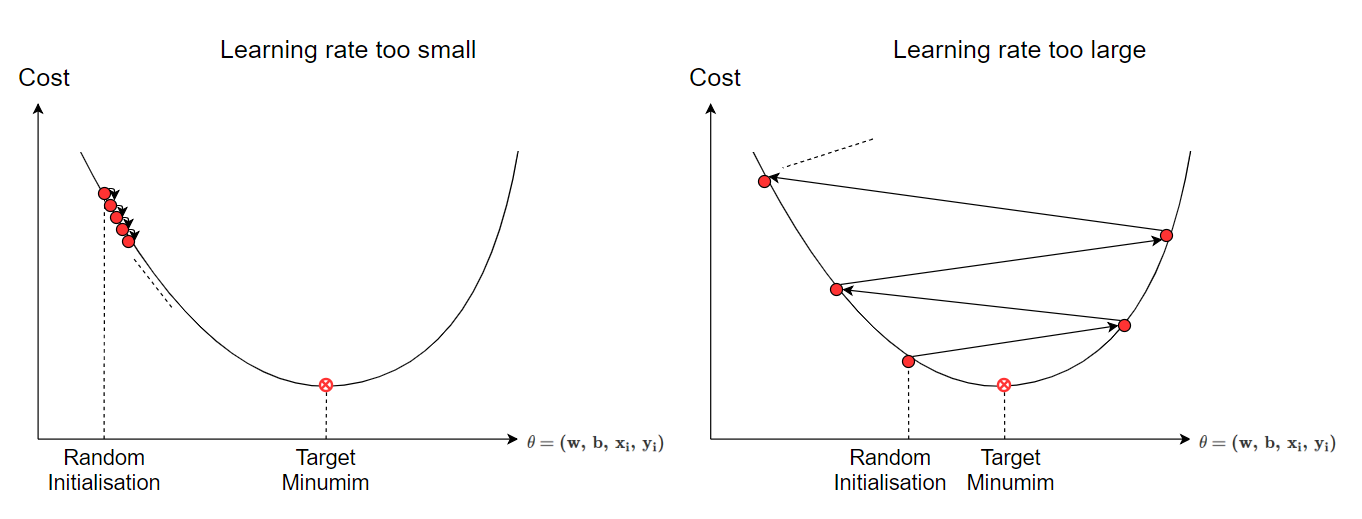
\includegraphics[scale = 0.5]{Images/learningrate.png}
  \caption{Gradient Descent behaviour depending on learning rate.}
  \label{learnrate}
\end{figure}



The backpropagation algorithm$^{\small \cite{backprop}}$ is now used to evaluate the partial derivatives, which can intuitively be interpreted as the gradient of the loss function, defined in the equations above. It starts from the final layer of the NN and computes the gradient directly from the loss function. Afterwards, it uses the chain rule to compute the gradient at each layer from the next layer until in reaches the input layer. \\



\subsubsection*{Predicting}

A trained model used on unseen data returns a prediction y. This can be used to estimate the class the input \textbf{x} lays in.

\begin{equation}
  c = \argmax_{c \in \{ c_1, c_2, ..., c_k\}} \ \mathbb{P}(\mathbf{x} \ \text{in class} \ c_i) = \argmax_{i \in \{ 1, 2, ..., k\}} \ y_i
\end{equation}

\smallskip

\section{Introduction to Patchy-San}

\section{Baseline Models}

This section briefly presents the theoretical background behind the classification models for which off-the-shelf implementations were used, serving as baselines for the context classification pipeline architecture. 

\subsection{K-Nearest Neighbours Classifier}
Many classification approaches attempt to estimate the conditional distribution of Y (output probabilities) given X (input features), and then classify a given observation to the class with highest estimated probability. One such method is the K-nearest neighbors (KNN) classifier$^{\small \cite{KNN}}$. Given a positive integer K and a test observation x$_0$, the KNN classifier first identifies the neighbours K points in the training data that are closest to x$_0$, represented by N$_0$. It then estimates the conditional probability for class $j$ as the fraction of points in N$_0$ whose response values equal $j$:

\begin{equation}
    Pr(Y = j|X = x_0) = \frac{1}{K} \sum_{i \in N_0} I(y_i = j)
\end{equation}

Finally, KNN applies Bayes rule and classifies the test observation x$_0$ to
the class with the largest probability. \\

In other words, KNN estimates how likely a data point is to be a member of one group or the other depending on what group the data points nearest to it are in. A worth noting aspect of KNN is that it is an example of a \textit{lazy learner} algorithm, meaning that it does not build a model using the training set until a query of the data set is performed, as opposed to the NN approaches later presented. \\




\subsection{Random Forest Classifier}

A decision tree$^{\small \cite{decision_tree}}$ is a classifier expressed as a recursive partition of the instance space. The decision tree consists of nodes that form a rooted tree. In a decision tree, each internal node splits the instance space into two or more sub-spaces according to a certain discrete function of the input attributes values. In the simplest and most frequent case each test considers a single attribute, such that the instance space is partitioned according to the attribute’s value. Each leaf is assigned to one class representing the most appropriate target value. Alternatively, the leaf may hold a probability vector indicating the probability of the target attribute having a certain value. Instances are classified by navigating them from the root of the tree down to a leaf, according to the outcome of the tests along the path. \\

Random forest classifier$^{\small \cite{RF}}$ creates a set of decision trees from randomly selected subset of training set. It then aggregates the votes from different decision trees to decide the final class of the test object. \\

\section{Requirement Analysis} \label{Requirement Analysis}

After performing an extensive inspection into the NN background theory, a decision was to be made regarding how to approach an implementation that satisfies the end goal of the project. Therefore, to build a ML pipeline capable of classifying, renaming and reorganising files in terms of both provenance and content information, a list of necessary steps is presented in Table \ref{Requirements overview}. \bigskip

\begin{longtable}{|p{.50\textwidth}|p{.15\textwidth}|p{.15\textwidth}|p{.15\textwidth}|}
  \hline
  \textbf{Requirements}                                        & \textbf{Priority} & \textbf{Risk} & \textbf{Difficulty} \\
  \hline
  Dataset understanding and investigation of existing patterns & High              & Low           & Low                 \\

  Receptive fields construction using Patchy-SAN               & High              & Low           & Medium              \\

  CNN implementation                                           & High              & Medium        & High                \\

  Generate synthetic data                                      & Medium            & Medium        & Medium              \\

  Hyperparameter tuning                                        & Medium            & Medium        & High                \\

  ML pipeline service time evaluation                          & Medium            & Medium        & Medium              \\

  Files renaming and reorganising implementation               & Low               & Medium        & Medium              \\

  \hline
  \caption[Requirements overview]{List of requirements for a successful project implementation, alongside with their risks and difficulties.}
  \label{Requirements overview}
\end{longtable} \bigskip


\section{Choice of Tools}

\subsection{Programming Languages}

I use Python 3.6.7 as the main programming language for building my project. This choice is sustained by the fact that Python provides an extensive selection of libraries and frameworks that facilitate deep learning algorithms implementation. Moreover, its syntax simplicity and high-quality documentation enhanced my experience throughout the development process. \\\

As a secondary programming language, I used Cypher Data Manipulation Language to interact with the original provided data set, which is stored as a graph database in Neo4J.

\subsection{Libraries}

The third-party libraries that were used alongside Python Standard Library are listed in Table \ref{Libraries}. \bigskip

\begin{longtable}{|p{.15\textwidth}|p{.10\textwidth}|p{.60\textwidth}|}
  \hline
  \textbf{Library} & \textbf{Version} & \textbf{Description}                                                                                                                                  \\
  \hline
  neo4j-driver     & 1.6.2            & Querying Neo4J graph database                                                                                                                         \\

  numpy            & 1.16.0           & Adds support for multi-dimensional arrays and matrices, along with a large collection of high-level mathematical functions to operate on these arrays \\

  sklearn          & 0.20.2           & Machine learning library                                                                                                                              \\

  networkx         & 2.2              & Used for for the creation, manipulation, and study of the structure, dynamics, and functions of complex networks                                      \\
  nauty            & 0.6.0            & Used for computing automorphism groups of graphs                                                                                                      \\

  matplotlib       & 3.0.2            & Data visualisation                                                                                                                                    \\


  \hline
  \caption[Libraries]{Third-party libraries used within project implementation.}
  \label{Libraries}
\end{longtable} \bigskip

\subsection{Development Environment}

Implementation, testing and evaluation of the project were performed on my personal machine (i7-6700HQ CPU 2.60GHz, 16GB RAM, 512GB SSD,  Ubuntu 18.04 LTS). Additionally, more resource intensive evaluations were carried out on GPUs provided by the Computer Laboratory Department. In terms of IDEs, I chose \textbf{PyCharm} due to its version control integration, on-the-fly error checking, debugging capabilities, flexibility and easy project navigation. \\\

To avoid possible issues created by either hardware/software failures or user errors, I had to place emphasis on adequately choosing backup strategies for my project. Thus, the git repository of the project was synchronised with \textbf{GitHub} online hosting service. The code was also occasionally updated on my Google Drive file space and on an external HDD. \\

\section{Starting Point}

I have started this project only having programming experience in C/C++ and Java. Thus, transition to Python was not problematic, as I had already covered fundamental concepts such as object-oriented and procedural programming. However, the more complicated stage was getting acquainted to the high-level NN APIs in Python. I needed to understand how to build NNs using off-the-shelf implementations for various layers, how to train, evaluate and optimise them. \\\

Moreover, I had only basic knowledge of machine learning. Part IA Machine Learning and Real World Data introduced the ideas of supervised learning and diverse evaluation metrics and strategies. However, additional preparation was needed to learn how NNs work, how to design their architecture, which regularisation techniques to use and what types would be most suitable for the project. \\

\section{Software Engineering Techniques}

Since all the requirements were clearly defined and understood, and also given the scale of the project, I decided to adopt the Iterative Development Model$^{\small \cite{iterative_model}}$. Respecting the concepts behind this software engineering model, I split my project into several modules that at first offer core functionality and are afterwards iteratively refined. The three indicated modules
consist of: database interaction module, machine learning pipeline module and a virtual filespace in which files are renamed and reorganised. \\\

Unit and integration testing were performed using (smaller) synthetically generated datasets. The datasets' generation tool gives the user full control over the way in which properties are generated and thus I could create similar patters to those in the original provenance graphs. \\

\section{Summary}

In this chapter, I introduced the neural networks background theory that supports the machine learning models built in the project, followed by analysing the requirements for achieving the success criteria and a brief description of the development environment and backup strategies. Furthermore, a software engineering model that describes how the project was step-by-step implemented and evaluated was also discussed. \\

\end{document}